\documentclass[twoside]{book}

% Packages required by doxygen
\usepackage{calc}
\usepackage{doxygen}
\usepackage{graphicx}
\usepackage[utf8]{inputenc}
\usepackage{makeidx}
\usepackage{multicol}
\usepackage{multirow}
\usepackage{textcomp}
\usepackage[table]{xcolor}

% Font selection
\usepackage[T1]{fontenc}
\usepackage{mathptmx}
\usepackage[scaled=.90]{helvet}
\usepackage{courier}
\usepackage{amssymb}
\usepackage{sectsty}
\renewcommand{\familydefault}{\sfdefault}
\allsectionsfont{%
  \fontseries{bc}\selectfont%
  \color{darkgray}%
}
\renewcommand{\DoxyLabelFont}{%
  \fontseries{bc}\selectfont%
  \color{darkgray}%
}

% Page & text layout
\usepackage{geometry}
\geometry{%
  a4paper,%
  top=2.5cm,%
  bottom=2.5cm,%
  left=2.5cm,%
  right=2.5cm%
}
\tolerance=750
\hfuzz=15pt
\hbadness=750
\setlength{\emergencystretch}{15pt}
\setlength{\parindent}{0cm}
\setlength{\parskip}{0.2cm}
\makeatletter
\renewcommand{\paragraph}{%
  \@startsection{paragraph}{4}{0ex}{-1.0ex}{1.0ex}{%
    \normalfont\normalsize\bfseries\SS@parafont%
  }%
}
\renewcommand{\subparagraph}{%
  \@startsection{subparagraph}{5}{0ex}{-1.0ex}{1.0ex}{%
    \normalfont\normalsize\bfseries\SS@subparafont%
  }%
}
\makeatother

% Headers & footers
\usepackage{fancyhdr}
\pagestyle{fancyplain}
\fancyhead[LE]{\fancyplain{}{\bfseries\thepage}}
\fancyhead[CE]{\fancyplain{}{}}
\fancyhead[RE]{\fancyplain{}{\bfseries\leftmark}}
\fancyhead[LO]{\fancyplain{}{\bfseries\rightmark}}
\fancyhead[CO]{\fancyplain{}{}}
\fancyhead[RO]{\fancyplain{}{\bfseries\thepage}}
\fancyfoot[LE]{\fancyplain{}{}}
\fancyfoot[CE]{\fancyplain{}{}}
\fancyfoot[RE]{\fancyplain{}{\bfseries\scriptsize Generated on Wed Apr 24 2019 14\-:50\-:05 for My Project by Doxygen }}
\fancyfoot[LO]{\fancyplain{}{\bfseries\scriptsize Generated on Wed Apr 24 2019 14\-:50\-:05 for My Project by Doxygen }}
\fancyfoot[CO]{\fancyplain{}{}}
\fancyfoot[RO]{\fancyplain{}{}}
\renewcommand{\footrulewidth}{0.4pt}
\renewcommand{\chaptermark}[1]{%
  \markboth{#1}{}%
}
\renewcommand{\sectionmark}[1]{%
  \markright{\thesection\ #1}%
}

% Indices & bibliography
\usepackage{natbib}
\usepackage[titles]{tocloft}
\setcounter{tocdepth}{3}
\setcounter{secnumdepth}{5}
\makeindex

% Hyperlinks (required, but should be loaded last)
\usepackage{ifpdf}
\ifpdf
  \usepackage[pdftex,pagebackref=true]{hyperref}
\else
  \usepackage[ps2pdf,pagebackref=true]{hyperref}
\fi
\hypersetup{%
  colorlinks=true,%
  linkcolor=blue,%
  citecolor=blue,%
  unicode%
}

% Custom commands
\newcommand{\clearemptydoublepage}{%
  \newpage{\pagestyle{empty}\cleardoublepage}%
}


%===== C O N T E N T S =====

\begin{document}

% Titlepage & ToC
\hypersetup{pageanchor=false}
\pagenumbering{roman}
\begin{titlepage}
\vspace*{7cm}
\begin{center}%
{\Large My Project }\\
\vspace*{1cm}
{\large Generated by Doxygen 1.8.5}\\
\vspace*{0.5cm}
{\small Wed Apr 24 2019 14:50:05}\\
\end{center}
\end{titlepage}
\clearemptydoublepage
\tableofcontents
\clearemptydoublepage
\pagenumbering{arabic}
\hypersetup{pageanchor=true}

%--- Begin generated contents ---
\chapter{Hierarchical Index}
\section{Class Hierarchy}
This inheritance list is sorted roughly, but not completely, alphabetically\-:\begin{DoxyCompactList}
\item Bridge\begin{DoxyCompactList}
\item \contentsline{section}{Minecraft\-Proxy\-Encoder.\-Minecraft\-Proxy\-Bridge}{\pageref{classMinecraftProxyEncoder_1_1MinecraftProxyBridge}}{}
\end{DoxyCompactList}
\item Client\-Factory\begin{DoxyCompactList}
\item \contentsline{section}{Minecraft\-Client\-Encoder.\-Minecraft\-Encoder\-Factory}{\pageref{classMinecraftClientEncoder_1_1MinecraftEncoderFactory}}{}
\end{DoxyCompactList}
\item Downstream\-Factory\begin{DoxyCompactList}
\item \contentsline{section}{Minecraft\-Proxy\-Encoder.\-Minecraft\-Proxy\-Factory}{\pageref{classMinecraftProxyEncoder_1_1MinecraftProxyFactory}}{}
\end{DoxyCompactList}
\item Spawning\-Client\-Protocol\begin{DoxyCompactList}
\item \contentsline{section}{Minecraft\-Client\-Encoder.\-Minecraft\-Client\-Encoder}{\pageref{classMinecraftClientEncoder_1_1MinecraftClientEncoder}}{}
\end{DoxyCompactList}
\item Upstream\begin{DoxyCompactList}
\item \contentsline{section}{Minecraft\-Proxy\-Encoder.\-Upstream\-Encoder}{\pageref{classMinecraftProxyEncoder_1_1UpstreamEncoder}}{}
\end{DoxyCompactList}
\item Upstream\-Factory\begin{DoxyCompactList}
\item \contentsline{section}{Minecraft\-Proxy\-Encoder.\-Upstream\-Encoder\-Factory}{\pageref{classMinecraftProxyEncoder_1_1UpstreamEncoderFactory}}{}
\end{DoxyCompactList}
\end{DoxyCompactList}

\chapter{Class Index}
\section{Class List}
Here are the classes, structs, unions and interfaces with brief descriptions\-:\begin{DoxyCompactList}
\item\contentsline{section}{\hyperlink{classMinecraftClientEncoder_1_1MinecraftClientEncoder}{Minecraft\-Client\-Encoder.\-Minecraft\-Client\-Encoder} }{\pageref{classMinecraftClientEncoder_1_1MinecraftClientEncoder}}{}
\item\contentsline{section}{\hyperlink{classMinecraftClientEncoder_1_1MinecraftEncoderFactory}{Minecraft\-Client\-Encoder.\-Minecraft\-Encoder\-Factory} }{\pageref{classMinecraftClientEncoder_1_1MinecraftEncoderFactory}}{}
\item\contentsline{section}{\hyperlink{classMinecraftProxyEncoder_1_1MinecraftProxyBridge}{Minecraft\-Proxy\-Encoder.\-Minecraft\-Proxy\-Bridge} }{\pageref{classMinecraftProxyEncoder_1_1MinecraftProxyBridge}}{}
\item\contentsline{section}{\hyperlink{classMinecraftProxyEncoder_1_1MinecraftProxyFactory}{Minecraft\-Proxy\-Encoder.\-Minecraft\-Proxy\-Factory} }{\pageref{classMinecraftProxyEncoder_1_1MinecraftProxyFactory}}{}
\item\contentsline{section}{\hyperlink{classMinecraftProxyEncoder_1_1UpstreamEncoder}{Minecraft\-Proxy\-Encoder.\-Upstream\-Encoder} }{\pageref{classMinecraftProxyEncoder_1_1UpstreamEncoder}}{}
\item\contentsline{section}{\hyperlink{classMinecraftProxyEncoder_1_1UpstreamEncoderFactory}{Minecraft\-Proxy\-Encoder.\-Upstream\-Encoder\-Factory} }{\pageref{classMinecraftProxyEncoder_1_1UpstreamEncoderFactory}}{}
\end{DoxyCompactList}

\chapter{Class Documentation}
\hypertarget{classMinecraftClientEncoder_1_1MinecraftClientEncoder}{\section{Minecraft\-Client\-Encoder.\-Minecraft\-Client\-Encoder Class Reference}
\label{classMinecraftClientEncoder_1_1MinecraftClientEncoder}\index{Minecraft\-Client\-Encoder.\-Minecraft\-Client\-Encoder@{Minecraft\-Client\-Encoder.\-Minecraft\-Client\-Encoder}}
}
Inheritance diagram for Minecraft\-Client\-Encoder.\-Minecraft\-Client\-Encoder\-:\begin{figure}[H]
\begin{center}
\leavevmode
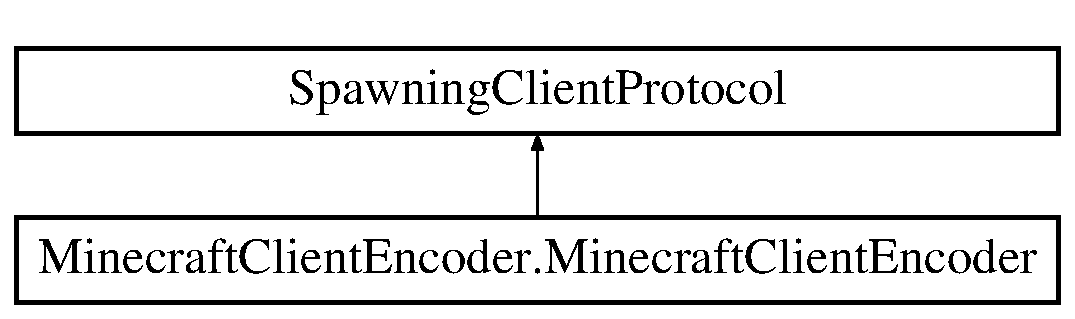
\includegraphics[height=2.000000cm]{classMinecraftClientEncoder_1_1MinecraftClientEncoder}
\end{center}
\end{figure}
\subsection*{Public Member Functions}
\begin{DoxyCompactItemize}
\item 
\hypertarget{classMinecraftClientEncoder_1_1MinecraftClientEncoder_a5301388bb9d010444b9e443f02700644}{def {\bfseries \-\_\-\-\_\-init\-\_\-\-\_\-}}\label{classMinecraftClientEncoder_1_1MinecraftClientEncoder_a5301388bb9d010444b9e443f02700644}

\item 
def \hyperlink{classMinecraftClientEncoder_1_1MinecraftClientEncoder_adcb6cbc129dd2550e43550130e2d9df4}{update\-\_\-player\-\_\-full}
\item 
\hypertarget{classMinecraftClientEncoder_1_1MinecraftClientEncoder_a8fa7df816f3cbd53b3b33d3f8410b69d}{def {\bfseries get\-\_\-byte\-\_\-from\-\_\-buff}}\label{classMinecraftClientEncoder_1_1MinecraftClientEncoder_a8fa7df816f3cbd53b3b33d3f8410b69d}

\item 
\hypertarget{classMinecraftClientEncoder_1_1MinecraftClientEncoder_aaec67d40f2f12790ba2eb80056d4dfac}{def {\bfseries get\-\_\-bytes\-\_\-from\-\_\-buff}}\label{classMinecraftClientEncoder_1_1MinecraftClientEncoder_aaec67d40f2f12790ba2eb80056d4dfac}

\item 
\hypertarget{classMinecraftClientEncoder_1_1MinecraftClientEncoder_ac0479e9e9e50e233b6760760e2f36086}{def {\bfseries check\-\_\-buff}}\label{classMinecraftClientEncoder_1_1MinecraftClientEncoder_ac0479e9e9e50e233b6760760e2f36086}

\item 
\hypertarget{classMinecraftClientEncoder_1_1MinecraftClientEncoder_a4fb9902dfc35420f15158fbe8fe66ef5}{def {\bfseries encode}}\label{classMinecraftClientEncoder_1_1MinecraftClientEncoder_a4fb9902dfc35420f15158fbe8fe66ef5}

\item 
\hypertarget{classMinecraftClientEncoder_1_1MinecraftClientEncoder_a5acf28fd1c6f249076dab2722ce2ef72}{def {\bfseries encode\-\_\-inventory\-\_\-action}}\label{classMinecraftClientEncoder_1_1MinecraftClientEncoder_a5acf28fd1c6f249076dab2722ce2ef72}

\item 
\hypertarget{classMinecraftClientEncoder_1_1MinecraftClientEncoder_ad3eb52ed31fba33e0d747735f5b2bfc9}{def {\bfseries encode\-\_\-player\-\_\-look}}\label{classMinecraftClientEncoder_1_1MinecraftClientEncoder_ad3eb52ed31fba33e0d747735f5b2bfc9}

\item 
\hypertarget{classMinecraftClientEncoder_1_1MinecraftClientEncoder_a3d5bc97e9e3799a8b05ed55f93120566}{def {\bfseries encode\-\_\-player\-\_\-position}}\label{classMinecraftClientEncoder_1_1MinecraftClientEncoder_a3d5bc97e9e3799a8b05ed55f93120566}

\item 
\hypertarget{classMinecraftClientEncoder_1_1MinecraftClientEncoder_ac53ed9c8f931ef5ed59efeb4d774ed04}{def {\bfseries encode\-\_\-player\-\_\-position\-\_\-and\-\_\-look}}\label{classMinecraftClientEncoder_1_1MinecraftClientEncoder_ac53ed9c8f931ef5ed59efeb4d774ed04}

\item 
\hypertarget{classMinecraftClientEncoder_1_1MinecraftClientEncoder_a39798d1a84a2d931c1e8cc13f8a245c3}{def {\bfseries packet\-\_\-player\-\_\-position\-\_\-and\-\_\-look}}\label{classMinecraftClientEncoder_1_1MinecraftClientEncoder_a39798d1a84a2d931c1e8cc13f8a245c3}

\item 
\hypertarget{classMinecraftClientEncoder_1_1MinecraftClientEncoder_a69016c89352da1024f9119da6da2c2eb}{def {\bfseries update\-\_\-incoming\-\_\-buffer}}\label{classMinecraftClientEncoder_1_1MinecraftClientEncoder_a69016c89352da1024f9119da6da2c2eb}

\item 
\hypertarget{classMinecraftClientEncoder_1_1MinecraftClientEncoder_afc8457a7dbfb5b7b662e739b217f8fdd}{def {\bfseries check\-\_\-entity}}\label{classMinecraftClientEncoder_1_1MinecraftClientEncoder_afc8457a7dbfb5b7b662e739b217f8fdd}

\item 
\hypertarget{classMinecraftClientEncoder_1_1MinecraftClientEncoder_a298643e416451d7d0f262d648e5f2050}{def {\bfseries packet\-\_\-entity\-\_\-head\-\_\-look}}\label{classMinecraftClientEncoder_1_1MinecraftClientEncoder_a298643e416451d7d0f262d648e5f2050}

\item 
\hypertarget{classMinecraftClientEncoder_1_1MinecraftClientEncoder_a892e1c6a02541ced5a938c2071f922b7}{def {\bfseries packet\-\_\-spawn\-\_\-mob}}\label{classMinecraftClientEncoder_1_1MinecraftClientEncoder_a892e1c6a02541ced5a938c2071f922b7}

\item 
\hypertarget{classMinecraftClientEncoder_1_1MinecraftClientEncoder_a0f438b44da1d60ceb50b4ab4b257a54a}{def {\bfseries packet\-\_\-entity\-\_\-relative\-\_\-move}}\label{classMinecraftClientEncoder_1_1MinecraftClientEncoder_a0f438b44da1d60ceb50b4ab4b257a54a}

\item 
\hypertarget{classMinecraftClientEncoder_1_1MinecraftClientEncoder_a21356b6feba28498608a6f4730b2c821}{def {\bfseries packet\-\_\-entity\-\_\-look}}\label{classMinecraftClientEncoder_1_1MinecraftClientEncoder_a21356b6feba28498608a6f4730b2c821}

\item 
\hypertarget{classMinecraftClientEncoder_1_1MinecraftClientEncoder_a9e13b791383cbb523fe54e6069c6396e}{def {\bfseries packet\-\_\-entity\-\_\-look\-\_\-and\-\_\-relative\-\_\-move}}\label{classMinecraftClientEncoder_1_1MinecraftClientEncoder_a9e13b791383cbb523fe54e6069c6396e}

\end{DoxyCompactItemize}
\subsection*{Public Attributes}
\begin{DoxyCompactItemize}
\item 
\hypertarget{classMinecraftClientEncoder_1_1MinecraftClientEncoder_a53b04bdfa4cdd62069c3820f2857cb1c}{{\bfseries packet\-\_\-done}}\label{classMinecraftClientEncoder_1_1MinecraftClientEncoder_a53b04bdfa4cdd62069c3820f2857cb1c}

\item 
\hypertarget{classMinecraftClientEncoder_1_1MinecraftClientEncoder_afac133089623be73a6943c54566bf2bc}{{\bfseries A\-E\-S\-\_\-\-Block\-\_\-\-Len}}\label{classMinecraftClientEncoder_1_1MinecraftClientEncoder_afac133089623be73a6943c54566bf2bc}

\item 
\hypertarget{classMinecraftClientEncoder_1_1MinecraftClientEncoder_ac4b272d95cdae84b1280e16d02982dd8}{{\bfseries out\-\_\-enc\-\_\-buff}}\label{classMinecraftClientEncoder_1_1MinecraftClientEncoder_ac4b272d95cdae84b1280e16d02982dd8}

\item 
\hypertarget{classMinecraftClientEncoder_1_1MinecraftClientEncoder_a0d9cd7f868b90abbb49d4a7f906be042}{{\bfseries in\-\_\-enc\-\_\-buff}}\label{classMinecraftClientEncoder_1_1MinecraftClientEncoder_a0d9cd7f868b90abbb49d4a7f906be042}

\item 
\hypertarget{classMinecraftClientEncoder_1_1MinecraftClientEncoder_a03ab57b5815555859a5a416b63d68c8f}{{\bfseries pos\-\_\-look}}\label{classMinecraftClientEncoder_1_1MinecraftClientEncoder_a03ab57b5815555859a5a416b63d68c8f}

\item 
\hypertarget{classMinecraftClientEncoder_1_1MinecraftClientEncoder_abf192278a0ebc8bfdf83a5c3dc2d9d62}{{\bfseries spawned}}\label{classMinecraftClientEncoder_1_1MinecraftClientEncoder_abf192278a0ebc8bfdf83a5c3dc2d9d62}

\end{DoxyCompactItemize}


\subsection{Detailed Description}
\begin{DoxyVerb}The MinecraftClient Encoder is a class that represents a Minecraft Client connection and performs the FTE encoding of an encrypted bit stream.
\end{DoxyVerb}
 

\subsection{Member Function Documentation}
\hypertarget{classMinecraftClientEncoder_1_1MinecraftClientEncoder_adcb6cbc129dd2550e43550130e2d9df4}{\index{Minecraft\-Client\-Encoder\-::\-Minecraft\-Client\-Encoder@{Minecraft\-Client\-Encoder\-::\-Minecraft\-Client\-Encoder}!update\-\_\-player\-\_\-full@{update\-\_\-player\-\_\-full}}
\index{update\-\_\-player\-\_\-full@{update\-\_\-player\-\_\-full}!MinecraftClientEncoder::MinecraftClientEncoder@{Minecraft\-Client\-Encoder\-::\-Minecraft\-Client\-Encoder}}
\subsubsection[{update\-\_\-player\-\_\-full}]{\setlength{\rightskip}{0pt plus 5cm}def Minecraft\-Client\-Encoder.\-Minecraft\-Client\-Encoder.\-update\-\_\-player\-\_\-full (
\begin{DoxyParamCaption}
\item[{}]{self}
\end{DoxyParamCaption}
)}}\label{classMinecraftClientEncoder_1_1MinecraftClientEncoder_adcb6cbc129dd2550e43550130e2d9df4}
\begin{DoxyVerb}Sends a player's position to the server every 20 ticks (1 second).        \end{DoxyVerb}
 

The documentation for this class was generated from the following file\-:\begin{DoxyCompactItemize}
\item 
Minecraft\-Client\-Encoder.\-py\end{DoxyCompactItemize}

\hypertarget{classMinecraftClientEncoder_1_1MinecraftEncoderFactory}{\section{Minecraft\-Client\-Encoder.\-Minecraft\-Encoder\-Factory Class Reference}
\label{classMinecraftClientEncoder_1_1MinecraftEncoderFactory}\index{Minecraft\-Client\-Encoder.\-Minecraft\-Encoder\-Factory@{Minecraft\-Client\-Encoder.\-Minecraft\-Encoder\-Factory}}
}
Inheritance diagram for Minecraft\-Client\-Encoder.\-Minecraft\-Encoder\-Factory\-:\begin{figure}[H]
\begin{center}
\leavevmode
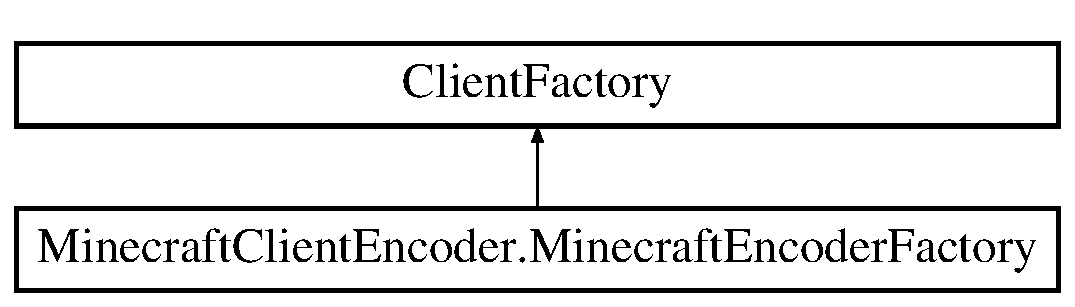
\includegraphics[height=2.000000cm]{classMinecraftClientEncoder_1_1MinecraftEncoderFactory}
\end{center}
\end{figure}
\subsection*{Public Member Functions}
\begin{DoxyCompactItemize}
\item 
\hypertarget{classMinecraftClientEncoder_1_1MinecraftEncoderFactory_a60c49451628cb91310196165946f7a68}{def {\bfseries \-\_\-\-\_\-init\-\_\-\-\_\-}}\label{classMinecraftClientEncoder_1_1MinecraftEncoderFactory_a60c49451628cb91310196165946f7a68}

\end{DoxyCompactItemize}
\subsection*{Public Attributes}
\begin{DoxyCompactItemize}
\item 
\hypertarget{classMinecraftClientEncoder_1_1MinecraftEncoderFactory_a3b3ef7e7fc4c0cd649445da12d0a8bb6}{{\bfseries forwarding\-\_\-packet\-\_\-queue}}\label{classMinecraftClientEncoder_1_1MinecraftEncoderFactory_a3b3ef7e7fc4c0cd649445da12d0a8bb6}

\item 
\hypertarget{classMinecraftClientEncoder_1_1MinecraftEncoderFactory_aef65b8ba462d9ea2d51dcf3d9713fd45}{{\bfseries receiving\-\_\-packet\-\_\-queue}}\label{classMinecraftClientEncoder_1_1MinecraftEncoderFactory_aef65b8ba462d9ea2d51dcf3d9713fd45}

\end{DoxyCompactItemize}
\subsection*{Static Public Attributes}
\begin{DoxyCompactItemize}
\item 
\hypertarget{classMinecraftClientEncoder_1_1MinecraftEncoderFactory_a6a94c5dbd65bda20f39399acdb9de9e9}{{\bfseries protocol} = \hyperlink{classMinecraftClientEncoder_1_1MinecraftClientEncoder}{Minecraft\-Client\-Encoder}}\label{classMinecraftClientEncoder_1_1MinecraftEncoderFactory_a6a94c5dbd65bda20f39399acdb9de9e9}

\end{DoxyCompactItemize}


\subsection{Detailed Description}
\begin{DoxyVerb}Factory for building Client Connections. Also serves as the interface
for the two packet queues for encoded packets being set between the
client and server of the Pluggable Transport.
\end{DoxyVerb}
 

The documentation for this class was generated from the following file\-:\begin{DoxyCompactItemize}
\item 
Minecraft\-Client\-Encoder.\-py\end{DoxyCompactItemize}

\hypertarget{classMinecraftProxyEncoder_1_1MinecraftProxyBridge}{\section{Minecraft\-Proxy\-Encoder.\-Minecraft\-Proxy\-Bridge Class Reference}
\label{classMinecraftProxyEncoder_1_1MinecraftProxyBridge}\index{Minecraft\-Proxy\-Encoder.\-Minecraft\-Proxy\-Bridge@{Minecraft\-Proxy\-Encoder.\-Minecraft\-Proxy\-Bridge}}
}
Inheritance diagram for Minecraft\-Proxy\-Encoder.\-Minecraft\-Proxy\-Bridge\-:\begin{figure}[H]
\begin{center}
\leavevmode
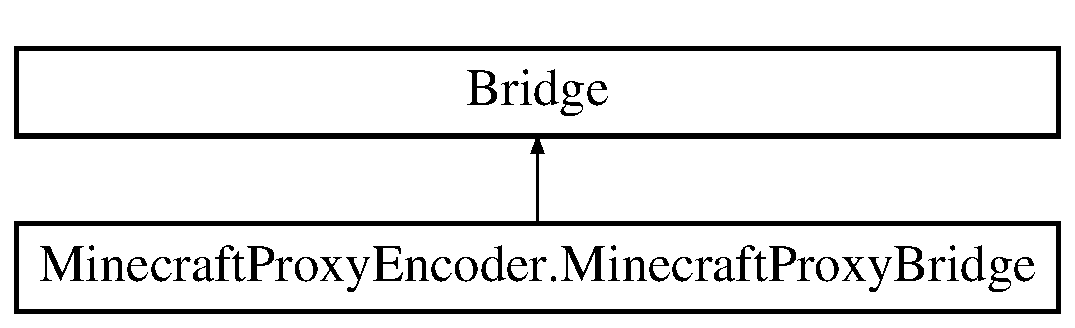
\includegraphics[height=2.000000cm]{classMinecraftProxyEncoder_1_1MinecraftProxyBridge}
\end{center}
\end{figure}
\subsection*{Public Member Functions}
\begin{DoxyCompactItemize}
\item 
\hypertarget{classMinecraftProxyEncoder_1_1MinecraftProxyBridge_a59a87a8587e75a8dc0d8fee09ec5ab4f}{def {\bfseries \-\_\-\-\_\-init\-\_\-\-\_\-}}\label{classMinecraftProxyEncoder_1_1MinecraftProxyBridge_a59a87a8587e75a8dc0d8fee09ec5ab4f}

\item 
\hypertarget{classMinecraftProxyEncoder_1_1MinecraftProxyBridge_a930c1973b8606605d967d5bb617ba2f0}{def {\bfseries get\-\_\-byte\-\_\-from\-\_\-buff}}\label{classMinecraftProxyEncoder_1_1MinecraftProxyBridge_a930c1973b8606605d967d5bb617ba2f0}

\item 
\hypertarget{classMinecraftProxyEncoder_1_1MinecraftProxyBridge_a1b55e4514a71e6105251a07bb1e9d940}{def {\bfseries get\-\_\-bytes\-\_\-from\-\_\-buff}}\label{classMinecraftProxyEncoder_1_1MinecraftProxyBridge_a1b55e4514a71e6105251a07bb1e9d940}

\item 
\hypertarget{classMinecraftProxyEncoder_1_1MinecraftProxyBridge_abfdd9c790d188e7bf1e6b83cc9341afa}{def {\bfseries check\-\_\-buff}}\label{classMinecraftProxyEncoder_1_1MinecraftProxyBridge_abfdd9c790d188e7bf1e6b83cc9341afa}

\item 
\hypertarget{classMinecraftProxyEncoder_1_1MinecraftProxyBridge_a4ba0539aa96aa3e824888adfaca2fdee}{def {\bfseries encode}}\label{classMinecraftProxyEncoder_1_1MinecraftProxyBridge_a4ba0539aa96aa3e824888adfaca2fdee}

\item 
\hypertarget{classMinecraftProxyEncoder_1_1MinecraftProxyBridge_a234339ff04992f59204e8837c3bc6c69}{def {\bfseries enemy\-\_\-enc\-\_\-head\-\_\-look}}\label{classMinecraftProxyEncoder_1_1MinecraftProxyBridge_a234339ff04992f59204e8837c3bc6c69}

\item 
\hypertarget{classMinecraftProxyEncoder_1_1MinecraftProxyBridge_a0b3121cb3c2498e0105cb1eaa17c917b}{def {\bfseries gen\-\_\-rand}}\label{classMinecraftProxyEncoder_1_1MinecraftProxyBridge_a0b3121cb3c2498e0105cb1eaa17c917b}

\item 
\hypertarget{classMinecraftProxyEncoder_1_1MinecraftProxyBridge_a1efbcc5a61e3a217967cb89b747aef4d}{def {\bfseries enemy\-\_\-enc\-\_\-look}}\label{classMinecraftProxyEncoder_1_1MinecraftProxyBridge_a1efbcc5a61e3a217967cb89b747aef4d}

\item 
\hypertarget{classMinecraftProxyEncoder_1_1MinecraftProxyBridge_a686bc748ed4fc584953119caddec78cf}{def {\bfseries spawn\-\_\-mobs}}\label{classMinecraftProxyEncoder_1_1MinecraftProxyBridge_a686bc748ed4fc584953119caddec78cf}

\item 
\hypertarget{classMinecraftProxyEncoder_1_1MinecraftProxyBridge_a0ef9c0d340e37441d3f09fc9e1386feb}{def {\bfseries update\-\_\-incoming\-\_\-buffer}}\label{classMinecraftProxyEncoder_1_1MinecraftProxyBridge_a0ef9c0d340e37441d3f09fc9e1386feb}

\item 
\hypertarget{classMinecraftProxyEncoder_1_1MinecraftProxyBridge_a4f6625b7cef14987f201927bcf4999de}{def {\bfseries packet\-\_\-upstream\-\_\-creative\-\_\-inventory\-\_\-action}}\label{classMinecraftProxyEncoder_1_1MinecraftProxyBridge_a4f6625b7cef14987f201927bcf4999de}

\item 
\hypertarget{classMinecraftProxyEncoder_1_1MinecraftProxyBridge_ac4d71f5236b6c540b152c0943ec36e0d}{def {\bfseries packet\-\_\-upstream\-\_\-player\-\_\-look}}\label{classMinecraftProxyEncoder_1_1MinecraftProxyBridge_ac4d71f5236b6c540b152c0943ec36e0d}

\item 
\hypertarget{classMinecraftProxyEncoder_1_1MinecraftProxyBridge_a835565f4a9a96a6ea358b39bddbe4876}{def {\bfseries packet\-\_\-upstream\-\_\-player\-\_\-position}}\label{classMinecraftProxyEncoder_1_1MinecraftProxyBridge_a835565f4a9a96a6ea358b39bddbe4876}

\item 
\hypertarget{classMinecraftProxyEncoder_1_1MinecraftProxyBridge_ab3876c6cc794e90468499dfac01b9d65}{def {\bfseries packet\-\_\-upstream\-\_\-player\-\_\-position\-\_\-and\-\_\-look}}\label{classMinecraftProxyEncoder_1_1MinecraftProxyBridge_ab3876c6cc794e90468499dfac01b9d65}

\item 
\hypertarget{classMinecraftProxyEncoder_1_1MinecraftProxyBridge_aab45b384f241d669460436fdca0a5617}{def {\bfseries packet\-\_\-downstream\-\_\-entity\-\_\-head\-\_\-look}}\label{classMinecraftProxyEncoder_1_1MinecraftProxyBridge_aab45b384f241d669460436fdca0a5617}

\item 
\hypertarget{classMinecraftProxyEncoder_1_1MinecraftProxyBridge_a974456aa0bb9ad839ca57cfa10ca7399}{def {\bfseries packet\-\_\-downstream\-\_\-entity\-\_\-look}}\label{classMinecraftProxyEncoder_1_1MinecraftProxyBridge_a974456aa0bb9ad839ca57cfa10ca7399}

\item 
\hypertarget{classMinecraftProxyEncoder_1_1MinecraftProxyBridge_a95cff10c5de7adcac5df4979a6f9380d}{def {\bfseries packet\-\_\-downstream\-\_\-player\-\_\-position\-\_\-and\-\_\-look}}\label{classMinecraftProxyEncoder_1_1MinecraftProxyBridge_a95cff10c5de7adcac5df4979a6f9380d}

\item 
\hypertarget{classMinecraftProxyEncoder_1_1MinecraftProxyBridge_aa59f2c29153f2871771c2406a0b805b4}{def {\bfseries downstream\-\_\-disconnected}}\label{classMinecraftProxyEncoder_1_1MinecraftProxyBridge_aa59f2c29153f2871771c2406a0b805b4}

\end{DoxyCompactItemize}
\subsection*{Public Attributes}
\begin{DoxyCompactItemize}
\item 
\hypertarget{classMinecraftProxyEncoder_1_1MinecraftProxyBridge_aba3a3b18503e841f796ca37fa06887fe}{{\bfseries clients\-\_\-and\-\_\-positions}}\label{classMinecraftProxyEncoder_1_1MinecraftProxyBridge_aba3a3b18503e841f796ca37fa06887fe}

\item 
\hypertarget{classMinecraftProxyEncoder_1_1MinecraftProxyBridge_a3c63d5f3e22a2280c7337e3e8376eda4}{{\bfseries out\-\_\-enc\-\_\-buff}}\label{classMinecraftProxyEncoder_1_1MinecraftProxyBridge_a3c63d5f3e22a2280c7337e3e8376eda4}

\item 
\hypertarget{classMinecraftProxyEncoder_1_1MinecraftProxyBridge_a64eef85735d58ad7010e97e1332ead29}{{\bfseries old\-\_\-enc\-\_\-buff}}\label{classMinecraftProxyEncoder_1_1MinecraftProxyBridge_a64eef85735d58ad7010e97e1332ead29}

\item 
\hypertarget{classMinecraftProxyEncoder_1_1MinecraftProxyBridge_af5d255a9d828c3dafc46289320c3dadf}{{\bfseries mobs\-\_\-per\-\_\-client}}\label{classMinecraftProxyEncoder_1_1MinecraftProxyBridge_af5d255a9d828c3dafc46289320c3dadf}

\item 
\hypertarget{classMinecraftProxyEncoder_1_1MinecraftProxyBridge_aa813423ec8189453e2b6f133581cd005}{{\bfseries first\-\_\-enemy\-\_\-id}}\label{classMinecraftProxyEncoder_1_1MinecraftProxyBridge_aa813423ec8189453e2b6f133581cd005}

\item 
\hypertarget{classMinecraftProxyEncoder_1_1MinecraftProxyBridge_ac418b92168c3d0db91b4304853cad0cf}{{\bfseries packet\-\_\-done}}\label{classMinecraftProxyEncoder_1_1MinecraftProxyBridge_ac418b92168c3d0db91b4304853cad0cf}

\item 
\hypertarget{classMinecraftProxyEncoder_1_1MinecraftProxyBridge_a466f0bcc02d954ade5febd0316709e4e}{{\bfseries is\-\_\-waiting}}\label{classMinecraftProxyEncoder_1_1MinecraftProxyBridge_a466f0bcc02d954ade5febd0316709e4e}

\item 
\hypertarget{classMinecraftProxyEncoder_1_1MinecraftProxyBridge_af978a4ae3f469be94a0e9f35678f7ebb}{{\bfseries block\-\_\-len}}\label{classMinecraftProxyEncoder_1_1MinecraftProxyBridge_af978a4ae3f469be94a0e9f35678f7ebb}

\end{DoxyCompactItemize}
\subsection*{Static Public Attributes}
\begin{DoxyCompactItemize}
\item 
\hypertarget{classMinecraftProxyEncoder_1_1MinecraftProxyBridge_a64507dfd55d2b140bd6cf62b454c1d96}{{\bfseries quiet\-\_\-mode} = False}\label{classMinecraftProxyEncoder_1_1MinecraftProxyBridge_a64507dfd55d2b140bd6cf62b454c1d96}

\item 
\hypertarget{classMinecraftProxyEncoder_1_1MinecraftProxyBridge_a36cc22a3da768073ae0f5c64e16b9876}{{\bfseries events\-\_\-enabled} = False}\label{classMinecraftProxyEncoder_1_1MinecraftProxyBridge_a36cc22a3da768073ae0f5c64e16b9876}

\item 
\hypertarget{classMinecraftProxyEncoder_1_1MinecraftProxyBridge_a2ababd31cb2f72360d032b61720dbcde}{{\bfseries upstream\-\_\-factory\-\_\-class} = \hyperlink{classMinecraftProxyEncoder_1_1UpstreamEncoderFactory}{Upstream\-Encoder\-Factory}}\label{classMinecraftProxyEncoder_1_1MinecraftProxyBridge_a2ababd31cb2f72360d032b61720dbcde}

\end{DoxyCompactItemize}


The documentation for this class was generated from the following file\-:\begin{DoxyCompactItemize}
\item 
Minecraft\-Proxy\-Encoder.\-py\end{DoxyCompactItemize}

\hypertarget{classMinecraftProxyEncoder_1_1MinecraftProxyFactory}{\section{Minecraft\-Proxy\-Encoder.\-Minecraft\-Proxy\-Factory Class Reference}
\label{classMinecraftProxyEncoder_1_1MinecraftProxyFactory}\index{Minecraft\-Proxy\-Encoder.\-Minecraft\-Proxy\-Factory@{Minecraft\-Proxy\-Encoder.\-Minecraft\-Proxy\-Factory}}
}
Inheritance diagram for Minecraft\-Proxy\-Encoder.\-Minecraft\-Proxy\-Factory\-:\begin{figure}[H]
\begin{center}
\leavevmode
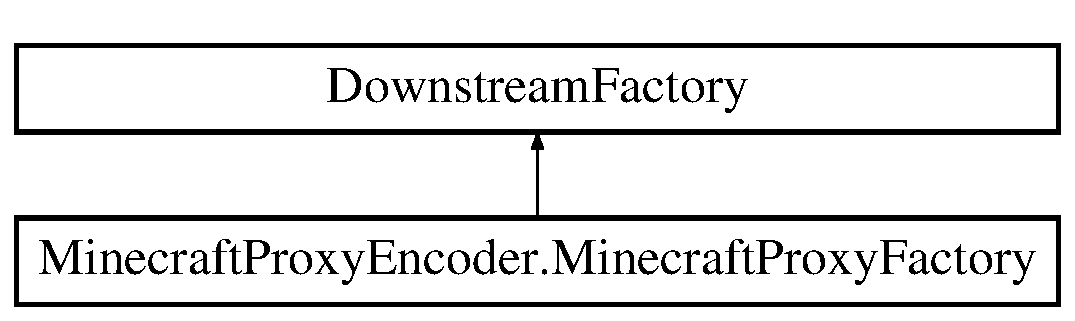
\includegraphics[height=2.000000cm]{classMinecraftProxyEncoder_1_1MinecraftProxyFactory}
\end{center}
\end{figure}
\subsection*{Public Member Functions}
\begin{DoxyCompactItemize}
\item 
\hypertarget{classMinecraftProxyEncoder_1_1MinecraftProxyFactory_ada29cb19ac42324305975b278c95e27e}{def {\bfseries \-\_\-\-\_\-init\-\_\-\-\_\-}}\label{classMinecraftProxyEncoder_1_1MinecraftProxyFactory_ada29cb19ac42324305975b278c95e27e}

\item 
\hypertarget{classMinecraftProxyEncoder_1_1MinecraftProxyFactory_ab3cd1d406e7d7bd7663df559aade3b94}{def {\bfseries connection\-Made}}\label{classMinecraftProxyEncoder_1_1MinecraftProxyFactory_ab3cd1d406e7d7bd7663df559aade3b94}

\item 
\hypertarget{classMinecraftProxyEncoder_1_1MinecraftProxyFactory_a2d37171bf0d968dd0ddedff9fb50e847}{def {\bfseries sync\-\_\-buff}}\label{classMinecraftProxyEncoder_1_1MinecraftProxyFactory_a2d37171bf0d968dd0ddedff9fb50e847}

\end{DoxyCompactItemize}
\subsection*{Public Attributes}
\begin{DoxyCompactItemize}
\item 
\hypertarget{classMinecraftProxyEncoder_1_1MinecraftProxyFactory_adb21e6de649b79302b77b972077a6d6b}{{\bfseries receiving\-\_\-packet\-\_\-queue}}\label{classMinecraftProxyEncoder_1_1MinecraftProxyFactory_adb21e6de649b79302b77b972077a6d6b}

\item 
\hypertarget{classMinecraftProxyEncoder_1_1MinecraftProxyFactory_a98df7277709c81ae6217fe1fc8c548e0}{{\bfseries num\-\_\-client\-\_\-encoders}}\label{classMinecraftProxyEncoder_1_1MinecraftProxyFactory_a98df7277709c81ae6217fe1fc8c548e0}

\item 
\hypertarget{classMinecraftProxyEncoder_1_1MinecraftProxyFactory_ad5b9bfc8cee927782d50af1645f6af80}{{\bfseries num\-\_\-waiting\-\_\-encoders}}\label{classMinecraftProxyEncoder_1_1MinecraftProxyFactory_ad5b9bfc8cee927782d50af1645f6af80}

\item 
\hypertarget{classMinecraftProxyEncoder_1_1MinecraftProxyFactory_acc52d45e71b462775cb479a4f88ae4ce}{{\bfseries out\-\_\-enc\-\_\-buff}}\label{classMinecraftProxyEncoder_1_1MinecraftProxyFactory_acc52d45e71b462775cb479a4f88ae4ce}

\end{DoxyCompactItemize}
\subsection*{Static Public Attributes}
\begin{DoxyCompactItemize}
\item 
\hypertarget{classMinecraftProxyEncoder_1_1MinecraftProxyFactory_a16144e5f1caf08c9bc6396380726bada}{{\bfseries bridge\-\_\-class} = \hyperlink{classMinecraftProxyEncoder_1_1MinecraftProxyBridge}{Minecraft\-Proxy\-Bridge}}\label{classMinecraftProxyEncoder_1_1MinecraftProxyFactory_a16144e5f1caf08c9bc6396380726bada}

\item 
\hypertarget{classMinecraftProxyEncoder_1_1MinecraftProxyFactory_a5bdfd03a645f87a5a770c5c2db2de89b}{tuple {\bfseries out\-\_\-enc\-\_\-buff} = bytearray()}\label{classMinecraftProxyEncoder_1_1MinecraftProxyFactory_a5bdfd03a645f87a5a770c5c2db2de89b}

\item 
\hypertarget{classMinecraftProxyEncoder_1_1MinecraftProxyFactory_a10c3127c70951d77d35286af69479495}{int {\bfseries num\-\_\-client\-\_\-encoders} = 0}\label{classMinecraftProxyEncoder_1_1MinecraftProxyFactory_a10c3127c70951d77d35286af69479495}

\item 
\hypertarget{classMinecraftProxyEncoder_1_1MinecraftProxyFactory_ac16630c00870f6438365c686f9d8725a}{int {\bfseries num\-\_\-waiting\-\_\-encoders} = 0}\label{classMinecraftProxyEncoder_1_1MinecraftProxyFactory_ac16630c00870f6438365c686f9d8725a}

\item 
\hypertarget{classMinecraftProxyEncoder_1_1MinecraftProxyFactory_a0b1a71c543eb4aec0157b2d9ee542897}{string {\bfseries motd} = \char`\"{}Proxy Server\char`\"{}}\label{classMinecraftProxyEncoder_1_1MinecraftProxyFactory_a0b1a71c543eb4aec0157b2d9ee542897}

\item 
\hypertarget{classMinecraftProxyEncoder_1_1MinecraftProxyFactory_a6952a9c6fef1a9cafe035d4a6d0195b4}{{\bfseries forwarding\-\_\-packet\-\_\-queue} = None}\label{classMinecraftProxyEncoder_1_1MinecraftProxyFactory_a6952a9c6fef1a9cafe035d4a6d0195b4}

\end{DoxyCompactItemize}


The documentation for this class was generated from the following file\-:\begin{DoxyCompactItemize}
\item 
Minecraft\-Proxy\-Encoder.\-py\end{DoxyCompactItemize}

\hypertarget{classMinecraftProxyEncoder_1_1UpstreamEncoder}{\section{Minecraft\-Proxy\-Encoder.\-Upstream\-Encoder Class Reference}
\label{classMinecraftProxyEncoder_1_1UpstreamEncoder}\index{Minecraft\-Proxy\-Encoder.\-Upstream\-Encoder@{Minecraft\-Proxy\-Encoder.\-Upstream\-Encoder}}
}
Inheritance diagram for Minecraft\-Proxy\-Encoder.\-Upstream\-Encoder\-:\begin{figure}[H]
\begin{center}
\leavevmode
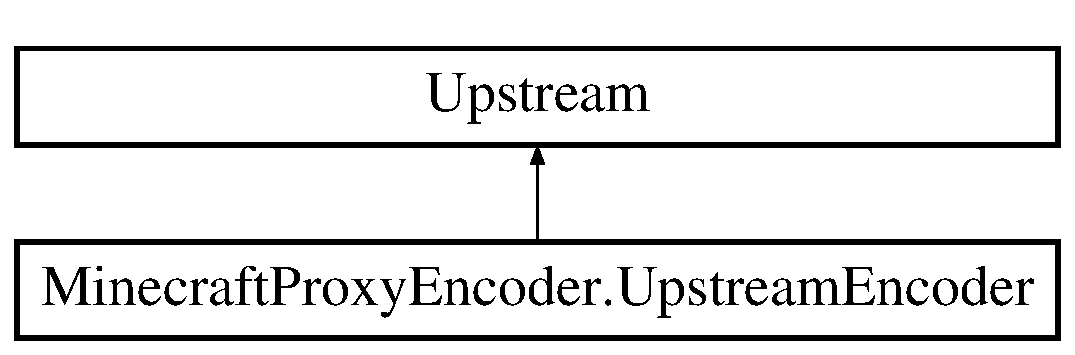
\includegraphics[height=2.000000cm]{classMinecraftProxyEncoder_1_1UpstreamEncoder}
\end{center}
\end{figure}
\subsection*{Static Public Attributes}
\begin{DoxyCompactItemize}
\item 
\hypertarget{classMinecraftProxyEncoder_1_1UpstreamEncoder_aaf9c962650494d59e02a19a5df0422f6}{tuple {\bfseries in\-\_\-enc\-\_\-buff} = bytearray()}\label{classMinecraftProxyEncoder_1_1UpstreamEncoder_aaf9c962650494d59e02a19a5df0422f6}

\item 
\hypertarget{classMinecraftProxyEncoder_1_1UpstreamEncoder_a8444207356e1b93746648e9796d1a7f7}{int {\bfseries assigned\-\_\-enemy} = 0}\label{classMinecraftProxyEncoder_1_1UpstreamEncoder_a8444207356e1b93746648e9796d1a7f7}

\item 
\hypertarget{classMinecraftProxyEncoder_1_1UpstreamEncoder_a011257181d74e8dceedfd403ac9594f5}{int {\bfseries assigned\-\_\-id} = 0}\label{classMinecraftProxyEncoder_1_1UpstreamEncoder_a011257181d74e8dceedfd403ac9594f5}

\end{DoxyCompactItemize}


The documentation for this class was generated from the following file\-:\begin{DoxyCompactItemize}
\item 
Minecraft\-Proxy\-Encoder.\-py\end{DoxyCompactItemize}

\hypertarget{classMinecraftProxyEncoder_1_1UpstreamEncoderFactory}{\section{Minecraft\-Proxy\-Encoder.\-Upstream\-Encoder\-Factory Class Reference}
\label{classMinecraftProxyEncoder_1_1UpstreamEncoderFactory}\index{Minecraft\-Proxy\-Encoder.\-Upstream\-Encoder\-Factory@{Minecraft\-Proxy\-Encoder.\-Upstream\-Encoder\-Factory}}
}
Inheritance diagram for Minecraft\-Proxy\-Encoder.\-Upstream\-Encoder\-Factory\-:\begin{figure}[H]
\begin{center}
\leavevmode
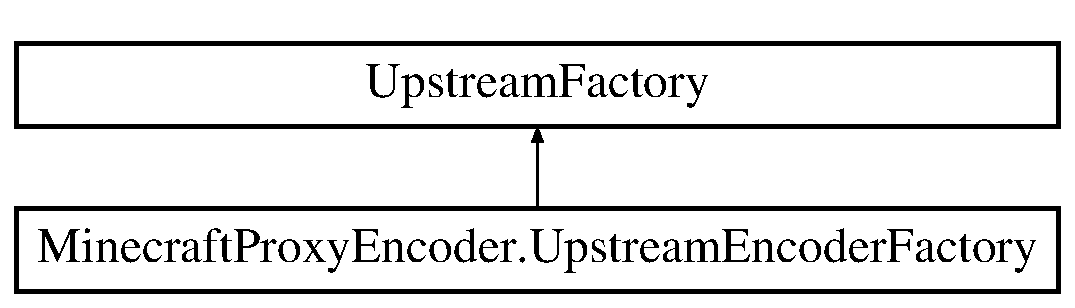
\includegraphics[height=2.000000cm]{classMinecraftProxyEncoder_1_1UpstreamEncoderFactory}
\end{center}
\end{figure}
\subsection*{Static Public Attributes}
\begin{DoxyCompactItemize}
\item 
\hypertarget{classMinecraftProxyEncoder_1_1UpstreamEncoderFactory_a0998ef42b6ade35b895175e7dc6100dd}{{\bfseries protocol} = \hyperlink{classMinecraftProxyEncoder_1_1UpstreamEncoder}{Upstream\-Encoder}}\label{classMinecraftProxyEncoder_1_1UpstreamEncoderFactory_a0998ef42b6ade35b895175e7dc6100dd}

\end{DoxyCompactItemize}


The documentation for this class was generated from the following file\-:\begin{DoxyCompactItemize}
\item 
Minecraft\-Proxy\-Encoder.\-py\end{DoxyCompactItemize}

%--- End generated contents ---

% Index
\newpage
\phantomsection
\addcontentsline{toc}{part}{Index}
\printindex

\end{document}
